\documentclass[10pt,conference]{IEEEtran}

%\usepackage[utf8]{inputenc}\usepackage[T1]{fontenc}
\usepackage{titling}
%\usepackage{times}
\setlength{\droptitle}{-5em}   % This is your set screw
\usepackage{ps2}
\usepackage{comment}
\usepackage{physics}
\usepackage{setspace}
\usepackage{bbm}
\usepackage{algorithm}
\usepackage{algorithmic}
\usepackage{etoolbox}
\AtBeginEnvironment{algorithm}{%
	\setlength{\columnwidth}{\linewidth}%
}
%\usepackage{titlesec}
%\titleformat{\section}{\large\bfseries}{\thesection}{1em}{}
\DeclareMathOperator{\interi}{int}
\DeclareMathOperator{\Clip}{clip}

\title{\bf\Large{Multi-Agent Area Coverage Control Using Reinforcement Learning}}
\author{Simon Hu}

\begin{document}
	
\maketitle
\thispagestyle{empty}
\pagestyle{empty}
\begin{abstract}
	In this paper, an area coverage control law is combined with a reinforcement learning algorithm to solve the optimal deployment problem. Traditional methods proposed for solving the method, from classical control theory, use proportional or linear quadratic Gaussian control designs. These traditional methods lack the robustness and adaptivity to dynamic environments, especially when these dynamic environment contribute significantly to the motion of the agents. A delayed actor-critic deep deterministic policy gradient algorithm is proposed to learn the value function and optimal policy. Simulation results are presented for stationary and time-varying scalar fields.
\end{abstract}
\section{Introduction}
	The problem of coverage control for multi-agent systems is concerned with deploying agents over an environment to maximize sensor coverage for various tasks like data collection and surveillance missions. Applications of this problem are harbour control, search and rescue, data, and surveillance missions. Consider a group of $N$ homogeneous agents moving in a compact environment $\Omega \subset \R^2$ where the dynamics of the $i$-th agent are given by 
	\begin{equation}
		\label{dynamics of robot}
		\displaystyle \ddot{p}_i = u_i
	\end{equation}
	where $p_i = (x_i, y_i)$ represents the agent's location and $u_i = (u_{x_i}, u_{y_i})$ represents the control input, which in this case is the direct acceleration input. The goal of solving the coverage control problem is to find the optimal configuration of the agent positions, $p = (p_1, p_2, \dots, p_N)$, with respect to the cost index
	\begin{equation}
		\label{cost function}
		\displaystyle \mathcal{H}(p, t) = \int_{\Omega}{\max\limits_{i=1,2,\dots,N}{f_i(\,\norm{q - p_i})}\phi(q,t) \: \dif q}
	\end{equation} 
	where the integral is understood in the sense of Lesbegue. In the above, $\phi: \Omega \times \R_{\geq 0} \to \R_{\geq 0}$ is a probibility density function that represents the probability of an event occuring at point $q \in \Omega$ and $f: \R^2 \to \R$ is a non-increasing function. Intuitively, $\phi(q,t)$ represents a belief of an event occuring at or near point $q$ at time $t$. The wider the spread around the point $q$, the more important it becomes for the agents to provide sensor coverage in that area. This density is either assumed to be known, or inferred using some other external algorithm. The function $f$ encodes the task to be performed. For the maximum area coverage problem, the function $f(x) = -x^2$ is used, and is assumed to be the same for all agents. It is easily checked that $f$ is measurable on $\Omega$ and is a non-increasing function.   
	\subsection{Voronoi Partitions}
		\begin{figure}
			\begin{subfigure}{0.2\textwidth}
				\centering 
				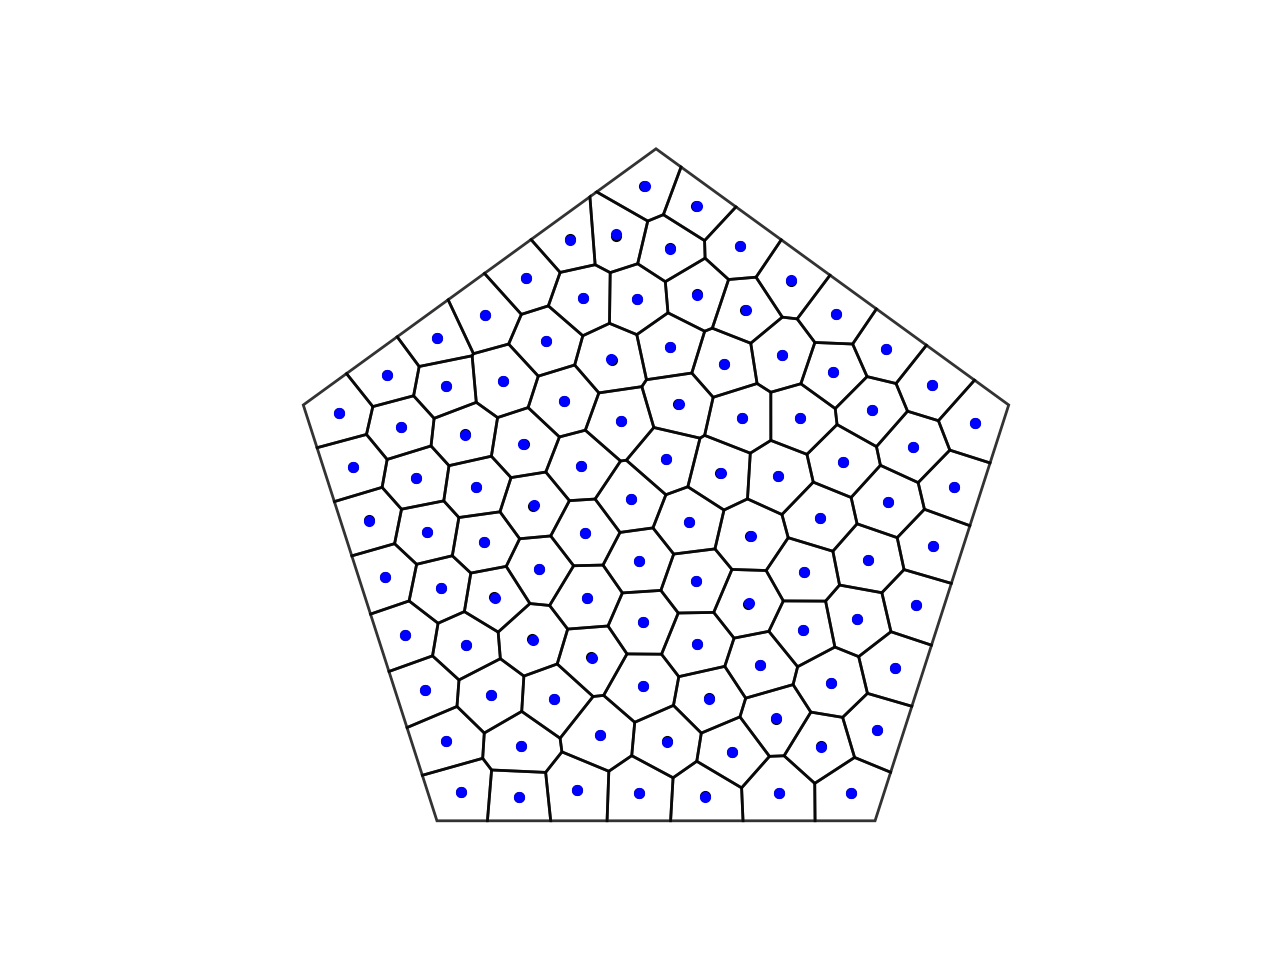
\includegraphics[scale=0.2]{fig_ex_2}
				\caption{}
			\end{subfigure}\hspace{\fill}
			\begin{subfigure}{0.2\textwidth}
				\centering 
				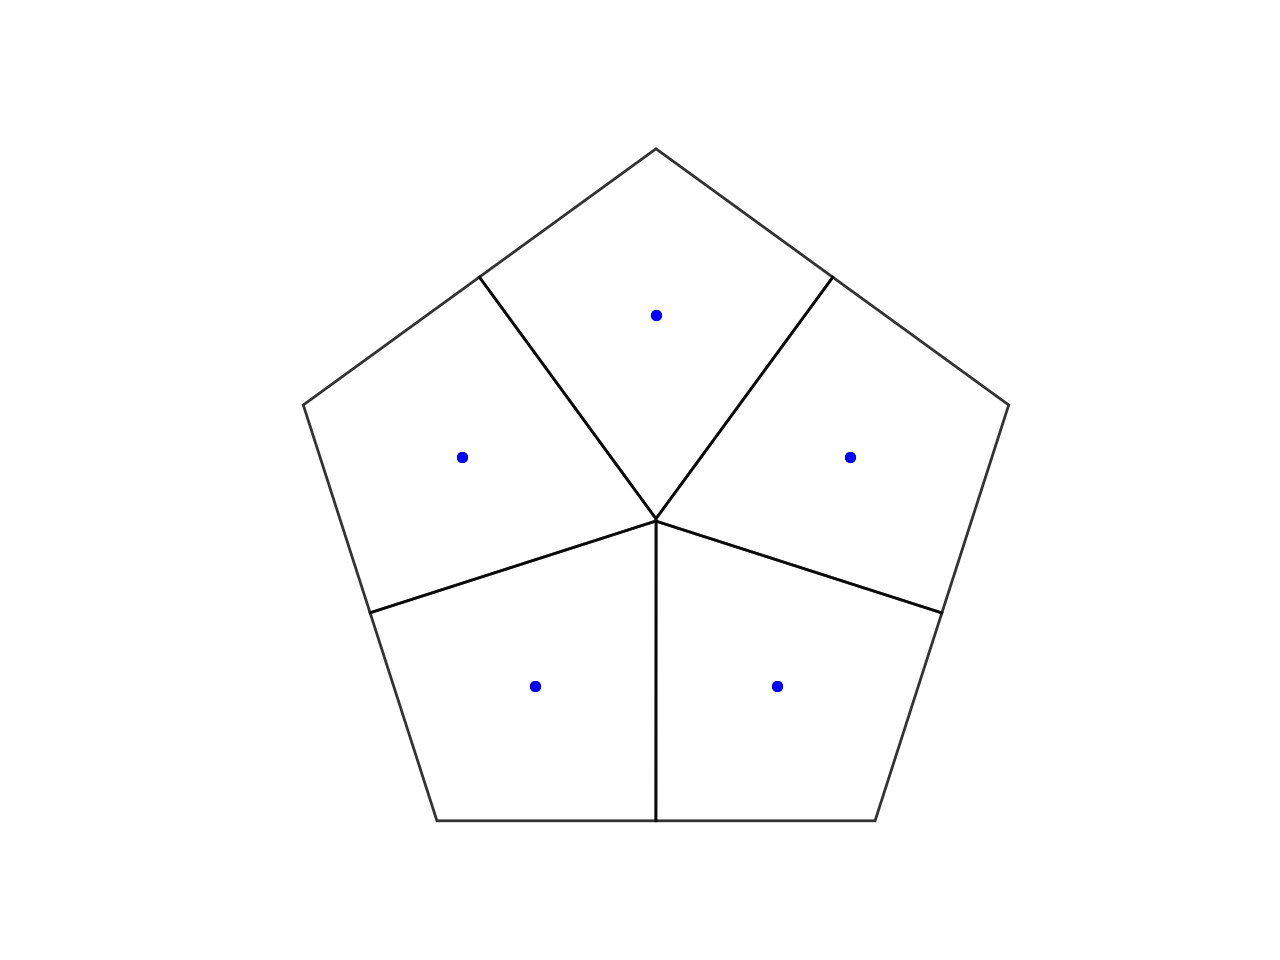
\includegraphics[scale=0.2]{fig_ex}
				\caption{}
			\end{subfigure}
			\caption{(a) An example of a Voronoi partition, assuming that $\phi$ is uniform and stationary. (b) An example of a centroidal Voronoi partition, assuming that $\phi$ is uniform and stationary.}
		\end{figure}
		A collection $S = (S_1, S_2, \dots, S_M)$ is a partition of $\Omega$ if each pair $(S_i, S_j)$ has disjoint interior and the union of all the $S_i$ is $\Omega$. That is, the $S_i$ cover $\Omega$. One particular partition of $\Omega$ is the Voronoi partition. The Voronoi partition of $\Omega$ is given by $V_{\Omega} = (\V_1, \V_2, \dots, \V_M)$ where each $V_i$ is given by 
		\begin{equation}
			\label{voronoi partitions}
			\displaystyle \V_i = \left\{ q \in \Omega \, : \, \norm{q - p_i} \leq \norm{q - p_j}, \, \forall j \neq i \right\}.
		\end{equation}
		We say that agents $i$ and $j$ are Voronoi neighbors if $\partial V_i \cap \partial \V_j \neq \emptyset$. That is, two agents are Voronoi neighbors if their Voronoi cells share a boundary. The mass and center of mass of a Voronoi cell are given by 
		\begin{align}
			\displaystyle &m_{\V_i} = \int_{\V_i}{\phi(q,t) \: \dif q} \\
			&c_{\V_i} = (m_{\V_i})^{-1}\int_{\V_i}{q\phi(q,t) \: \dif q}
		\end{align}
		respectively. The importance of the Voronoi partition framework is summarized in the following proposition. 
		\begin{prop}
			Let $V_\Omega$ be the Voronoi partition of $\Omega$. Then the cost index (\refeq{cost function}) can be rewritten as 
			\begin{equation}
				\label{cost function rewritten}
				\displaystyle \mathcal{H}(p, t) = \sum\limits_{i=1}^{N}{\int_{\V_i}{f(\, \norm{q - p_i}) \phi(q,t) \: \dif q}}.
			\end{equation}
		\end{prop}
		\begin{proof}
			Since $\V_\Omega$ is a covering of $\Omega$, we write (\refeq{cost function}) as 
			\begin{equation*}
				\displaystyle \mathcal{H}(p,t) = \sum\limits_{i=1}^{N}{\int_{\V_i}{\max\limits_{i=1,2,\dots,N}{f_i(\, \norm{q-p_i}) \phi(q,t) \: \dif q}}}.
			\end{equation*}
			The result then follows from the definition of $\V_i$ and the non-increasing property of $f$.
		\end{proof}
		The implications of proposition 1 are important to note. In many applications, agents must communicate with each other for various reasons. For example, consider a scenario where agents must communicate with each other for the purpose of avoiding collisions. Communications can be energy-intensive, unreliable, or impossible when the distance between agents is very large. However, proposition 1 implies that agent $i$ only needs to communicate with its Voronoi neighbors which reduces computational cost for communications at least, and makes the problem tractable at best. In this manner, any algorithm that utilizes the principle behind proposition $1$ is said to be spatially distributed with respect to the underlying distribution. 
	\subsection{Optimal Policy}
		It is shown in \cite{Cortes:2004} that the optimal partition of $\Omega$ is the centroidal Voronoi partition and the optimal sensor placement $p$ are located at the centers of the Voronoi cells. Thus, the optimal policy is to drive the agents towards their Voronoi centers. In \cite{Cortes:2004}, the authors consider a simple proportional-derivative controller of the form
		\begin{equation*}
			\displaystyle u_i = -k_p (c_{\V_i} - p_i) - k_d(\dot{c}_{\V_i} - \dot{p}_i)
		\end{equation*}
		where $k_p, k_d > 0$. This controller performs reasonably well. However, classical control methods requires either tuning sensitive hyperparameters, using integral control to account for different inputs, or a combination of both. Reinforcement learning methods are introduced to train agents that learn dynamics of themselves and the environment. This is especially inmportant in scenarios where agents are deployed over hydrodynamic or aerodynamic environments.  
\section{Technical Approach}
	Designing a controller that realizes the control law in \cite{Cortes:2004} is difficult, even for simple dynamics. When the dynamics become more intricate and complex, like an underwater glider dynamics for example, classical controller design becomes exponentially hard. To reduce this burden, reinforcement learning methodologies are employed. We first describe an actor-critic neural network approximation, and then an improvement to it, which is used in the final implementation. 
	\subsection{Actor-Critic DDPG}
	Define $e_i(t) = c_{\V_i}(t) - p_i(t)$ as the centroid error for agent $i$ and the Value function at the $k$-th step as
	\begin{equation}
		\label{value function}
		\displaystyle V(e_i(k)) = \sum\limits_{\kappa=k}^{\infty}{e_i^T(\kappa)Qe_i(\kappa) + u_i^T(\kappa)Ru_i(\kappa)}
	\end{equation}
	where $Q, R \in \R^{2\times 2}$ are positive definite matrices. Note that if the process noise is assumed to be Gaussian then this is just the linear quadratic regulartor design from classical control theory. The second term in (\refeq{value function}) encodes a measure of energy expenditure for physical systems so the design of the $R$ matrix is important for long-term surveillance and data collection tasks. For notational simplicity, we write $V_{i,k} = V_i(e_i(k))$. The value function is rewritten in the form of a Bellman equation, 
	\begin{equation}
		\displaystyle V_{i,k} = e_i^T(k)Qe_i(k) + u_i^T(k)Ru_i(k) + V_{i,k+1}
	\end{equation}
	so that the minimization problem to be solved is 
	\begin{equation*}
		\displaystyle V_{i,k}^* = \min\limits_{}{\left[ e_i^T(k)Qe_i(k) + u_i^T(k)Ru_i(k) + \gamma V_{i,k+1}^*\right]}
	\end{equation*}
	where $\gamma$ is the discount factor. The end goal is to use this value function to obtain a policy $\pi$ that ends up minimizing the value function. The authors in \cite{FLAIRS1612802} propose to use a neural network to approximate both the value function and the policy. They are assumed to take the structure 
	\begin{align}
		\displaystyle &\hat{V}_j(e_i(k)) = \omega_{c,j}^T \rho(e_i(k)), \\
		&\hat{\pi}_j(e_i(k)) = \omega_{a,j}^T\sigma(e_i(k)).
	\end{align}
	In the above, $\hat{V}_j$ and $\hat{\pi}_j$ are respectively the estimates of the value function and policy, $\omega_{c,j}, \omega_{a,j}$ are network weights at iteration $j$ and $\rho, \sigma$ are a series of activation functions from the neural network. The authors in \cite{FLAIRS1612802} consider a least-squares loss for both the actor and critic networks, but we use the MSE loss instead. 
	
	A target and source network are initialized and updated for both the actor and critic. The weights are synched using a soft update rule to improve numerical stability. A vanilla actor-critic DDPG algorithm (ACDDPG) is given in algorithm \refeq{acddpg}.
	\begin{algorithm}
		\caption{Actor-Critic DDPG (ACDDPG)}
		\begin{algorithmic}[1]
			\STATE Randomly initialize the critic network $Q(s, a|\theta^Q)$ and actor network $\pi(s|\theta^\mu)$ with weights $\theta_Q, \theta^\pi$. 
			\STATE Initialize a target network $Q'$ and $\pi'$ with the same weights as the networks above. 
			\STATE Initialize an empty replay buffer $R$.
			\FOR {episode = 1 \TO M} 
				\STATE Initialize a random process $\mathcal{N}$ for exploration. 
				\STATE Obtain an initial observation of the state, $s_1$. 
				\FOR {t = 1 \TO T}
					\STATE Select action $a_t = \pi(s_t|\theta^\mu) + \mathcal{N}_t$ according to the current policy and exploration noise.
					\STATE Execute action $a_t$ and observe the reward $r_t$ and new state $s_{t+1}$. 
					\STATE Store the transition dictionary $(s_t, a_t, r_t, s_{t+1})$ to $R$.
					\STATE Sample a minibatch of $N$ transitions $(s_i, a_i, r_i, s_{i+1})$ from $R$.
					\STATE Set $y_i = r_i + \gamma Q'(s_{i+1}, \pi'(s_{i+1}|\theta^{\pi'})|\theta^{Q'})$. 
					\STATE Update the critic network by minimizing the loss, given by equation (\refeq{critic_loss}).
					\STATE Update the actor network using the sampled policy gradient given by 
					\begin{equation*}
						\displaystyle \nabla_{\theta^\pi} J \approx \frac{1}{N}\sum\limits_{i}{\nabla_a Q(s,a|\theta^Q)|_{s - s_i, a = \pi(s_i)}\nabla_{\theta^\pi}\pi(s|\theta^\pi)|_{s_i}}.
					\end{equation*}
					\STATE Perform a soft update of the target networks:
					\begin{align*}
						&\theta^{Q'} \leftarrow \tau\theta^Q + (1-\tau)\theta^{Q'} \\
						&\theta^{\pi'} \leftarrow \tau \theta^\pi + (1-\tau)\theta^{\pi'}
					\end{align*}
				\ENDFOR
			\ENDFOR
		\end{algorithmic}
		\label{acddpg}
	\end{algorithm}
	\subsection{Twin-Delayed Soft Actor-Critic DDPG}
	The ACDDPG algorithm, while good, ends up most of the time overestimating the value function. The ACDDPG algorithm suffers from an overestimation of the value function. This overestimation propagates throughout the learning process and has a negative effect on the learned policy. This motivates the development of double Q-learning algorithms, where the action selection and Q-value updates are decoupled through the use of two value networks. In a setting like the ACDDPG algorithm, we keep track of two deterministic actors $\pi_{\theta_1}, \pi_{\theta_2}$ and two corresponding critics $Q_{\omega_1}, Q_{\omega_2}$ so that the Bellman updates are given by 
	\begin{align*}
		\displaystyle &y_1 = r + \gamma Q_{\omega_2}(s', \pi_{\theta_1}(s')), \\
		&y_2 = r + \gamma Q_{\omega_1}(s', \pi_{\theta_2}(s')).
	\end{align*}
	Clipped Q-learning, which uses the minimum estimated update between the two above, is applied so that the estimation of the value function is an underestimate. Biasing towards underestimation is preferred, since the underestimation of the value function is much harder to propagate through the learning process. The authors in \cite{fujimoto2018addressing} also consider a delayed soft-update of the network parameters, where the parameters of the policy are soft-updated at a lower frequency than the Q-function, so that the value function doesn't diverge when the estimate of the policy is poor. Finally, regularization is performed by adding a small amount of clipped noise to the action and updating is done in batches. With the clipping, the Bellman update takes the form
	\begin{equation*}
		\displaystyle y = r + \gamma Q_{\omega}(s', \pi_\theta(s') + \epsilon)
	\end{equation*}
	where $\epsilon \sim \Clip(\mathcal{N}(0, \sigma), -c, + c)$ is the clipped noise. The final twin-delayed actor-critic DDPG algorithm (TD3) is given in algorithm (cite here).
	\begin{algorithm}
		\caption{Twin-Delayed Actor-Critic DDPG (TD3)}
		\begin{algorithmic}[2]
			\STATE Initialize critic networks $Q_{\omega_1}, Q_{\omega_2}$ and actor network $\pi_{\theta}$ with random parameters
			$\omega_1, \omega_2, \theta$. 
			\STATE Initialize the target networks $\omega'_1 \leftarrow \omega_1, \omega'_2 \leftarrow \omega_2, \theta' \leftarrow \theta$.
			\STATE Initialize a replay buffer $R$.
			\FOR {$t = 1$ \TO $T$}
				\STATE Select action with exploration noise $a \sim \pi(s) + \epsilon, \epsilon \sim \mathcal{N}(0, \sigma)$ and record the reward $r$ and new state $s'$. 
				\STATE Store the tuple $(s, a, r, s')$ into $R$. 
				\STATE Sample minibatches of $N$ transitions $(s, a, r, s')$ from $R$.
				\STATE Smooth the target policy according to $\tilde{a} \leftarrow \pi_{\theta'}(s) + \epsilon, \epsilon \sim \Clip(\mathcal{N}(0, \tilde{\sigma}), -c, c)$.
				\STATE Clip the results according to the followng rule $y \leftarrow r + \gamma \min_{i=1,2}Q_{\omega'_i}(s', \tilde{a})$. 
				\STATE Update the critics according to $\omega_i \leftarrow \min_{\omega_i}N^{-1}\sum(y - Q_{\omega_i}(s, a))^2$.
				\IF {$t \mod d$} 
					\STATE Update $\theta$ by the deterministic policy gradient according to the following rule 
					\begin{equation*}
					\displaystyle \nabla_{\theta}J = N^{-1}\sum\nabla_a Q_{\omega_1}(s,a)\big|_{a = \pi_{\theta}}\nabla_{\theta}\pi_{\theta}.
					\end{equation*}
					\STATE Update the target networks according to 
					\begin{align*}
					\displaystyle &\omega'_i \leftarrow \tau\omega_i + (1-\tau)\omega'_i \\
					&\theta' \leftarrow \tau\theta + (1-\tau)\theta'.
					\end{align*}
				\ENDIF 
			\ENDFOR
		\end{algorithmic}
		\label{sacddpg}	
	\end{algorithm}
	\subsection{Multi-Agent Coverage Control Algorithm}
	Recall that the goal of area coverage is to maximize (\refeq{cost function}) by finding the optimal locations of the agents, $p$. Under the Voronoi partitions framework, it is shown in \cite{Cortes:2004} that the optimal configuration is obtained by iteratively having agents move to the centroids of their Voronoi cells. The proposed area coverage control algorithm uses the Voronoi framework and uses the TD3 algorithm to learn suitable controls for each agent. In essense, we combine the power of reinforcement learning with the Voronoi partitions framework to converge to the centroidal Voronoi configuration, which solves (\refeq{cost function}), in an optimal manner. 
	\section{Experimental Setup}
	We describe our experimental setup. This is composed of three main parts: an environment for training and simulations, an architecture for the neural network, and proposed scenarios. 
	\subsection{Environment}
		Training and simulations were performed on a custom-made environment. The environment is a two-dimensional pentagon whose convex hull is described by the vertices (insert vertices here). To make the simulations more 
\nocite{*}
\bibliography{ref}
\bibliographystyle{ieeetr}
\end{document}